\documentclass[11pt]{article}
\usepackage[utf8]{inputenc}
\usepackage[spanish]{babel}
\usepackage{graphicx}         % Para incluir imágenes
\usepackage{amsmath}          % Para notación matemática
\usepackage{amssymb}          % Para símbolos matemáticos como \mathbb
\usepackage[margin=3cm]{geometry}  % Márgenes
\usepackage[font=normalsize,labelfont=small]{caption}  % Estilo de captions
\usepackage{hyperref}         % Para links clickeables
\usepackage{textcomp}         % Para caracteres especiales
\usepackage{lmodern}          % Fuentes modernas con mejor soporte para caracteres
\usepackage{float}            % Para usar la opción H en figuras


% EXTENSIÓN MÁXIMA: 10 HOJAS SIN EXCEPCIÓN.
\begin{document}

\begin{titlepage}
    \centering
    \vspace*{2cm}
    
\includegraphics[scale=1.8]{Logo-Udesa.jpg}\par
    \vspace{10pt}

    {\LARGE \textbf{I302 - Aprendizaje Automático\\ y Aprendizaje Profundo}\par}
    \vspace{1cm}

    {\LARGE \textbf{Trabajo Práctico 4: \\Aprendizaje No-Supervisado}\par}
    \vspace{4cm}
    
    {\LARGE {Eliana  Ostrovsky}\par}  % <- Modificar Nombre y Apellido
    \vspace{4cm}
    
    {\Large \today\par}
    \vspace{1cm}
    \Large{Ingeniería en Inteligencia Artificial}
\end{titlepage}

% EJERCICIO 1
\section{Clustering de datos}
% INTRODUCCION

\subsection{Introducción}

El objetivo de este trabajo es aplicar técnicas de \textit{aprendizaje no supervisado} para analizar datos sin etiquetas previas mediante algoritmos de \textit{clustering}. En particular, se busca identificar estructuras y agrupamientos naturales dentro de un conjunto de datos provisto en el archivo \texttt{clustering.csv}.

El análisis se centra en tres algoritmos principales de agrupamiento: \textbf{K-means}, \textbf{Gaussian Mixture Models (GMM)} y \textbf{DBSCAN}. Cada uno de ellos presenta diferentes supuestos y estrategias para encontrar agrupaciones en los datos:
\begin{itemize}
    \item \textbf{K-means}: agrupa los datos en $K$ clusters minimizando la suma de distancias cuadráticas a los centroides, y requiere definir previamente la cantidad de clusters.
    \item \textbf{GMM}: extiende el enfoque de K-means permitiendo modelar cada cluster como una distribución gaussiana, lo que resulta útil para datos con formas más complejas.
    \item \textbf{DBSCAN}: permite encontrar clusters de forma arbitraria y detectar ruido, basándose en la densidad de los puntos.
\end{itemize}

La entrada para estos algoritmos consiste en un conjunto de datos con características numéricas representadas en dos dimensiones (es decir, puntos en el plano). El objetivo es determinar a qué agrupamiento pertenece cada punto, sin contar con etiquetas o clases previamente definidas. La salida esperada de cada algoritmo es una asignación de cada punto a un cluster (o, en el caso de DBSCAN, a ruido si corresponde), junto con los centroides o parámetros característicos de cada agrupación.

Este trabajo permite explorar las capacidades y limitaciones de cada técnica de clustering, comparando los resultados obtenidos y analizando su sensibilidad frente a parámetros como la cantidad de clusters (en K-means y GMM) o el radio de vecindad y densidad mínima (en DBSCAN).

\subsection{Métodos}

En este trabajo se implementaron tres algoritmos de agrupamiento no supervisado: \textbf{K-means}, \textbf{Gaussian Mixture Models (GMM)} y \textbf{DBSCAN}. A continuación se describen brevemente sus fundamentos y características.

\paragraph{K-means.} Este algoritmo particiona un conjunto de $n$ puntos $\{x_1, x_2, \dots, x_n\} \subset 
{R}^d$ en $K$ clusters. El objetivo es minimizar la suma de distancias cuadradas entre los puntos y el centroide de su cluster correspondiente. Formalmente, se busca minimizar la siguiente función de costo:

\[
L = \sum_{k=1}^{K} \sum_{x_i \in C_k} \|x_i - \mu_k\|^2
\]

donde $C_k$ es el conjunto de puntos asignados al cluster $k$ y $\mu_k$ es el centroide de dicho cluster. La cantidad $K$ se seleccionó utilizando el método del \textit{codo}, graficando la función $L(K)$ y observando el punto a partir del cual las ganancias por agregar clusters disminuyen significativamente.

\paragraph{Gaussian Mixture Models (GMM).} A diferencia de K-means, GMM modela la distribución de los datos como una combinación de $K$ distribuciones gaussianas. Cada cluster está representado por una gaussiana con media $\mu_k$ y covarianza $\Sigma_k$, y la probabilidad de cada punto está dada por:

\[
p(x_i) = \sum_{k=1}^K \pi_k \, \mathcal{N}(x_i \mid \mu_k, \Sigma_k)
\]

donde $\pi_k$ es el peso de la $k$-ésima componente. Los parámetros se estiman mediante el algoritmo de Expectation-Maximization (EM). La inicialización de GMM se realizó utilizando los centroides obtenidos con K-means para acelerar la convergencia.

\paragraph{DBSCAN.} Este algoritmo agrupa puntos basándose en la densidad local, definida a partir de un parámetro de vecindad $\varepsilon$ y un número mínimo de puntos $MinPts$. Un punto es considerado núcleo si tiene al menos $MinPts$ vecinos dentro de un radio $\varepsilon$. A partir de los núcleos se forman los clusters y los puntos que no pertenecen a ninguno se etiquetan como \textit{ruido}. DBSCAN no requiere especificar la cantidad de clusters, lo cual es útil para datos con formas arbitrarias o presencia de outliers. Se exploraron diferentes combinaciones de $\varepsilon$ y $MinPts$ para obtener una partición adecuada.

\paragraph{Datos y preprocesamiento.} El dataset \texttt{clustering.csv} contiene puntos bidimensionales $(x_1, x_2) \in \mathbb{R}^2$. Como se trata de un problema no supervisado, no se realizó una partición entrenamiento/validación/test. No se aplicó normalización adicional ya que las escalas eran comparables, pero se verificó la ausencia de valores faltantes o atípicos extremos antes del análisis.

\paragraph{Hiperparámetros.} Para K-means y GMM se exploraron valores de $K$ entre 1 y 20. Para DBSCAN se probaron distintos valores de $\varepsilon \in [20000, 22500, 25000, 27500]$ y $MinPts \in \{15, 20, 25, 30\}$, evaluando la calidad de los agrupamientos visualmente y mediante métricas internas.

\paragraph{Métricas.} Como el problema es no supervisado y no se dispone de etiquetas verdaderas, se utilizaron métricas internas para evaluar los agrupamientos: la \textbf{suma de distancias intra-cluster} (para K-means y GMM) y el \textbf{índice de silueta}, que mide cuán similar es un punto a su propio cluster en comparación con otros. También se evaluó visualmente la coherencia de los clusters obtenidos.

\subsection{Resultados}

A continuación se presentan los resultados obtenidos por los tres algoritmos implementados: K-means, Gaussian Mixture Models (GMM) y DBSCAN, aplicados al dataset \texttt{clustering.csv}.

\paragraph{K-means.} Se probó el algoritmo para diferentes valores de $K$ entre 1 y 20. La métrica utilizada fue la suma de distancias intra-cluster $L$, y se graficó $L$ en función de $K$ para aplicar el criterio del codo. El punto de inflexión se encontró en $K = 15$, indicando que ese valor representa un buen compromiso entre complejidad y calidad de agrupamiento (ver Figura~\ref{fig:kmeans_codo}). La Figura~\ref{fig:kmeans_clusters} muestra la asignación final de los puntos a los clusters y los centroides obtenidos.

\begin{figure}[H]
    \centering
    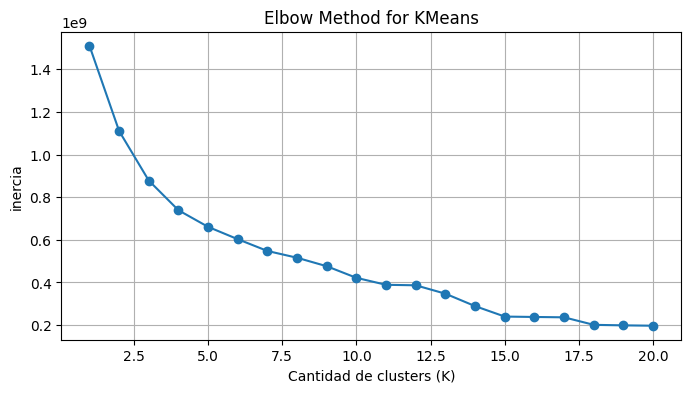
\includegraphics[width=0.6\textwidth]{figuras/kmeans_codo.png}
    \caption{Curva de la suma de distancias intra-cluster $L$ en función de $K$ (criterio del codo).}
    \label{fig:kmeans_codo}
\end{figure}

\begin{figure}[H]
    \centering
    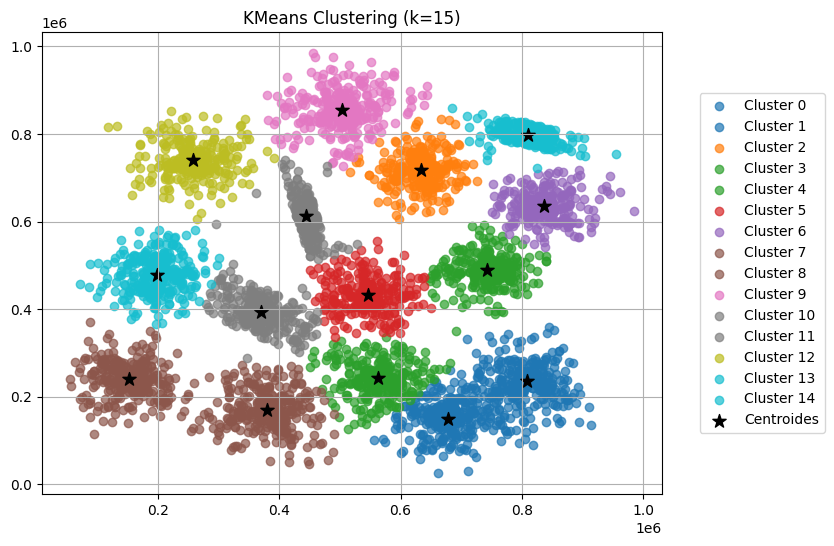
\includegraphics[width=0.6\textwidth]{figuras/kmeans_clusters.png}
    \caption{Clusters obtenidos con K-means ($K = 15$). Los centroides están marcados con un símbolo especial.}
    \label{fig:kmeans_clusters}
\end{figure}

\paragraph{GMM.} Se utilizó el mismo valor óptimo de $K = 15$ para inicializar el algoritmo GMM. La Figura~\ref{fig:gmm_clusters} muestra los clusters obtenidos. 

\begin{figure}[H]
    \centering
    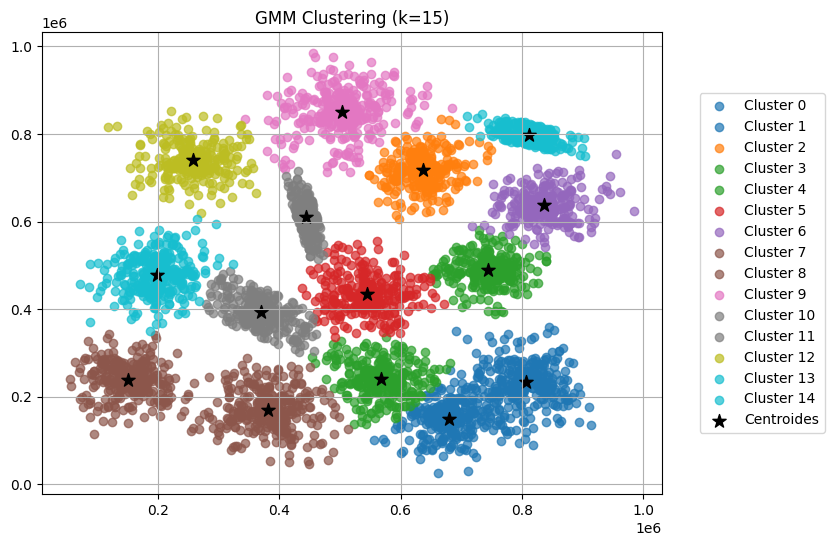
\includegraphics[width=0.6\textwidth]{figuras/gmm_clusters.png}
    \caption{Clusters obtenidos con Gaussian Mixture Models ($K = 15$).}
    \label{fig:gmm_clusters}
\end{figure}

\paragraph{DBSCAN.} A diferencia de los modelos anteriores, DBSCAN no requiere especificar $K$. Se exploraron distintos valores de $\varepsilon \in \{20000, 22500, 25000, 27500\}$ y $MinPts \in \{15, 20, 25, 30\}$. Para elegir se uso la metrica de silhouette ademas de la evaluacion visual.

\begin{figure}[H]
    \centering
    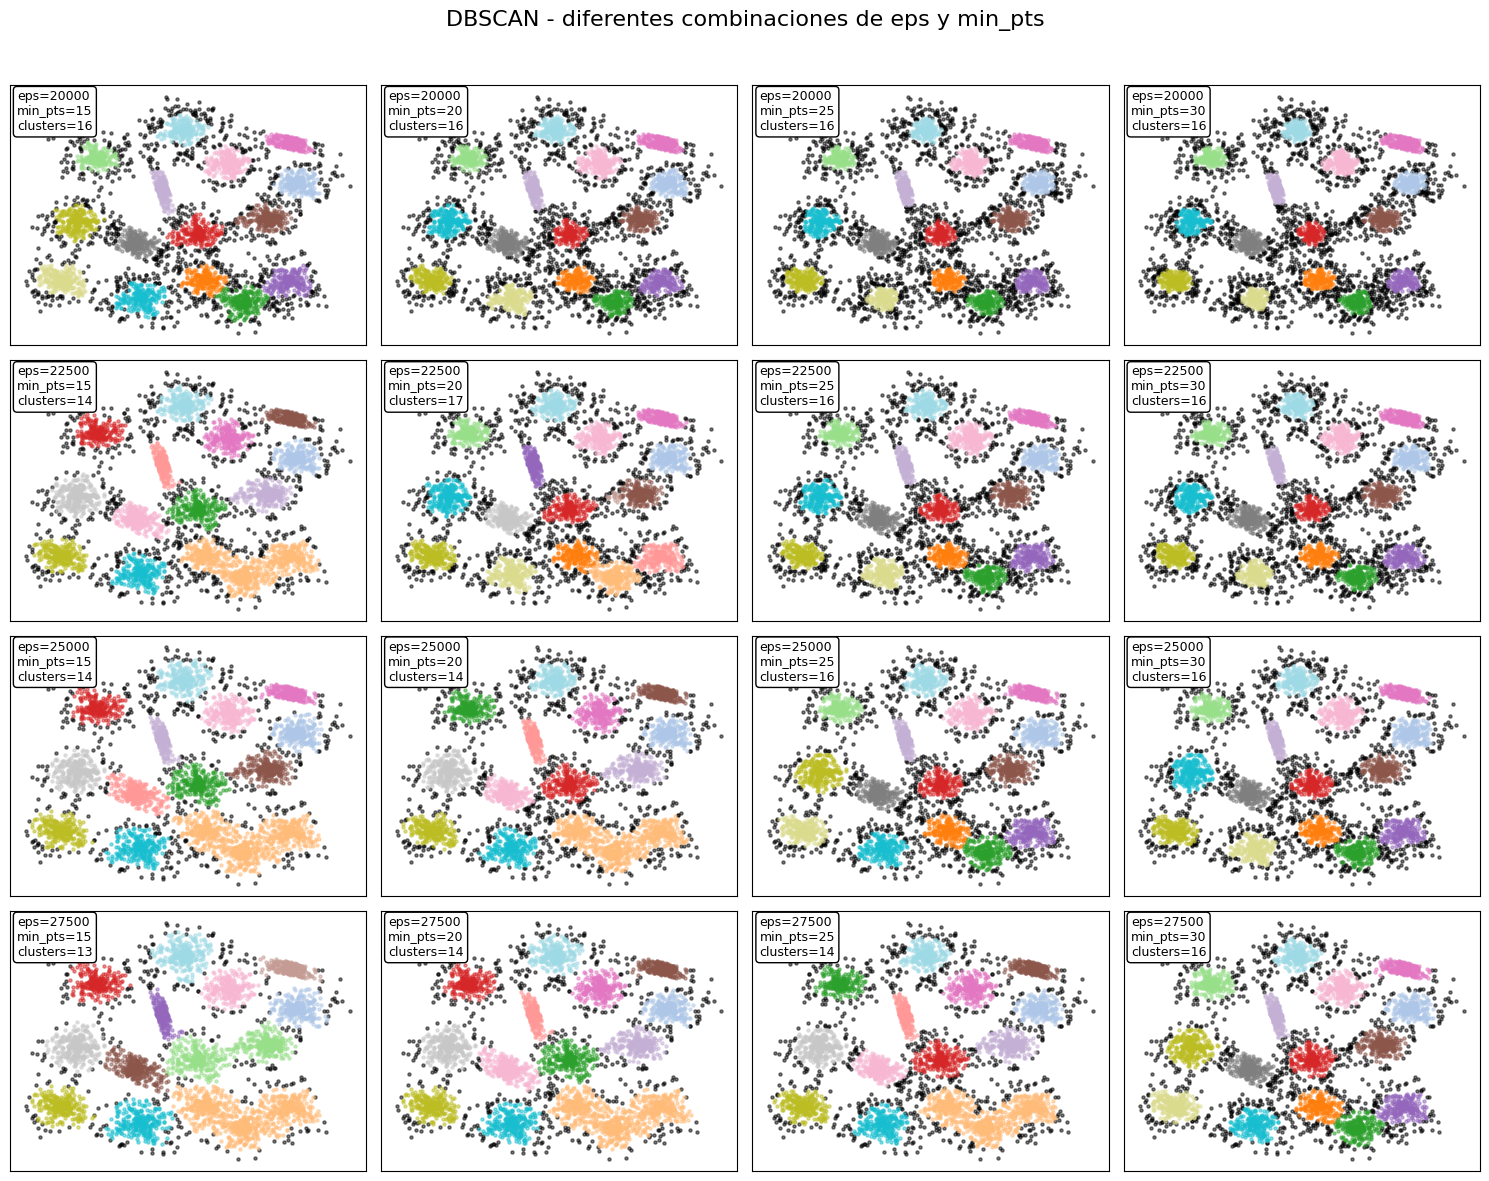
\includegraphics[width=0.8\textwidth]{figuras/dbscan_search.png}
    \caption{Los diferentes clusters obtenidos a partir del grid search de Hiperparámetros}
    \label{fig:dbscan_clusters}
\end{figure}

La mejor segmentación se obtuvo con $\varepsilon = 25000$ y $MinPts = 15$, logrando identificar correctamente agrupaciones no esféricas y puntos de ruido (ver Figura~\ref{fig:dbscan_clusters}). Si bien fue el más robusto frente a outliers, en ciertos casos pequeños cambios en los parámetros resultaron en una cantidad muy distinta de clusters.

\begin{figure}[H]
    \centering
    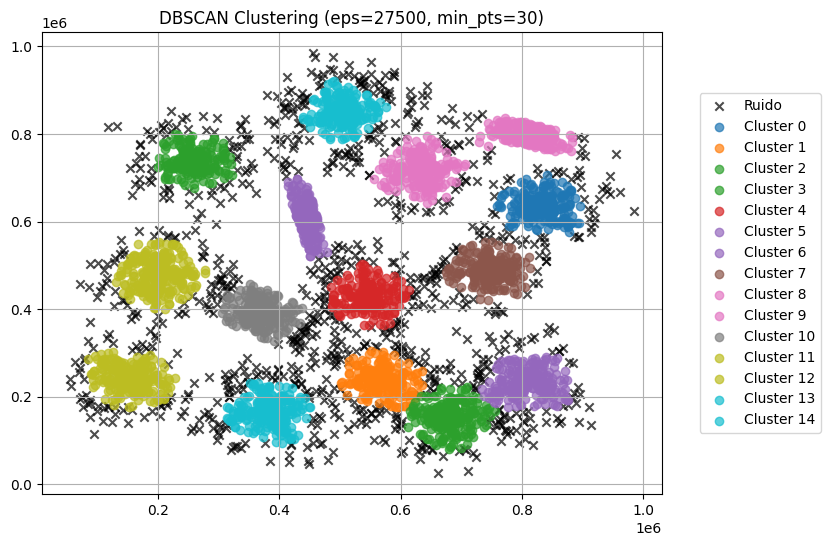
\includegraphics[width=0.6\textwidth]{figuras/dbscan_clusters.png}
    \caption{Clusters obtenidos con DBSCAN ($\varepsilon = 25000$, $MinPts = 15$). Los puntos clasificados como ruido están marcados en negro.}
    \label{fig:dbscan_clusters}
\end{figure}

% EJERCICIO 2
\section{Reducción de dimensionalidad}

\subsection{Introducción}

El objetivo de este ejercicio es aplicar técnicas de reducción de dimensionalidad para representar datos de alta dimensión en un espacio más compacto, preservando la mayor cantidad posible de información. En particular, se utilizó el algoritmo \textbf{Principal Component Analysis (PCA)} sobre el conjunto de datos \texttt{MNIST\_dataset.csv}, el cual contiene imágenes de dígitos del 0 al 9 representadas como vectores de 784 componentes (28x28 píxeles en escala de grises).

La entrada del algoritmo son vectores de intensidad de píxeles correspondientes a imágenes, y la salida son representaciones comprimidas con menor número de dimensiones (componentes principales), que permiten reconstruir aproximaciones de las imágenes originales o visualizar los datos en 2D. Esta reducción facilita el análisis y la visualización, y es útil como paso previo a tareas de clasificación o clustering.

\subsection{Métodos}

Se implementó el algoritmo de \textbf{PCA}, que consiste en encontrar una base ortogonal que maximiza la varianza de los datos proyectados. Formalmente, dado un conjunto de datos centrados $X \in \mathbb{R}^{n \times d}$, se calcula la matriz de covarianza $C = \frac{1}{n}X^\top X$, y luego se obtienen los autovalores $\lambda_i$ y autovectores $v_i$ de $C$. Las primeras $k$ componentes principales corresponden a los vectores $v_i$ asociados a los $k$ mayores autovalores.

El conjunto de datos original fue centrado respecto a la media. No se realizó partición entre entrenamiento y testeo dado que el objetivo es puramente exploratorio. Se evaluaron los errores de reconstrucción para diferentes valores de $k$, y también se graficó la varianza explicada acumulada.

La cantidad de componentes principales se eligió según el porcentaje de varianza acumulada que se desea preservar. Se calcularon los valores mínimos de $k$ necesarios para explicar el 90\%, 95\% y 99\% de la varianza.

\subsection{Resultados}

Se puede observar que existe una relación inversa entre la varianza explicada acumulada y el error cuadrático medio de reconstrucción: a medida que aumenta el número de componentes principales, la varianza explicada se incrementa mientras que el error de reconstrucción disminuye. Esta relación no es casual, ya que PCA tiene la propiedad matemática de que maximizar la varianza explicada es equivalente a minimizar el error cuadrático medio de reconstrucción.

\begin{figure}[H]
    \centering
    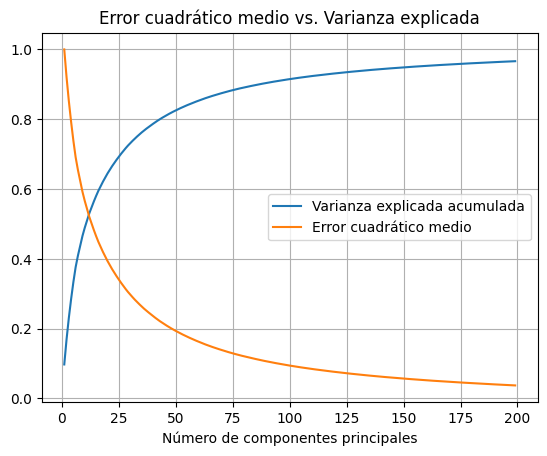
\includegraphics[width=0.5\textwidth]{figuras/pca_varianza_error.png}
    \caption{Error cuadrático medio en función del número de componentes principales.}
    \label{fig:pca_error}
\end{figure}

Para determinar el número óptimo de componentes principales, se buscó la cantidad mínima de dimensiones necesarias para explicar diferentes porcentajes de la varianza total de los datos. Se encontró que se necesitan aproximadamente $k=87$ componentes para explicar el 90\% de la varianza, $k=154$ componentes para el 95\%, y $k=331$ componentes para explicar el 99\% de la varianza total. Estos valores proporcionan puntos de referencia útiles para equilibrar la compresión de datos con la preservación de información, como se puede observar en la Figura~\ref{fig:pca_variance}.

\begin{figure}[H]
    \centering
    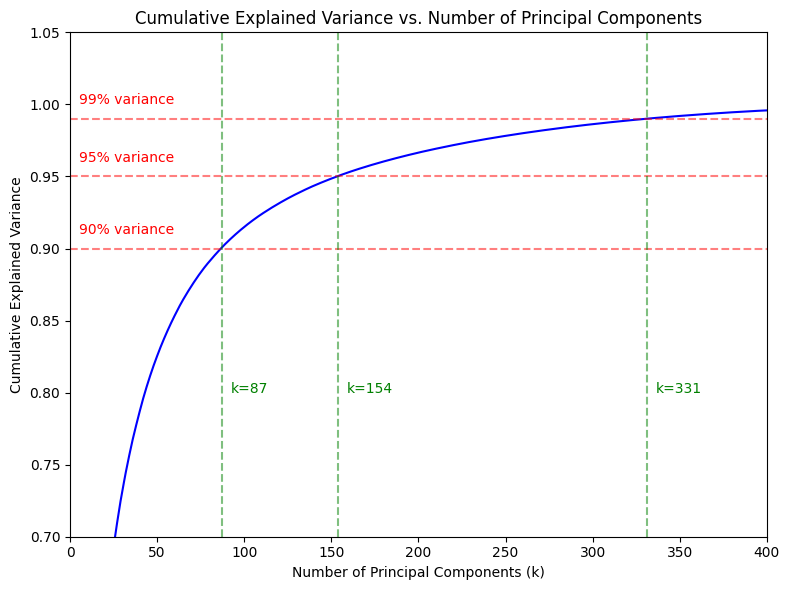
\includegraphics[width=0.7\textwidth]{figuras/varianzaexplicada.png}
    \caption{Varianza explicada acumulada en función del número de componentes principales.}
    \label{fig:pca_variance}
\end{figure}

La Figura~\ref{fig:pca_reconstructions} muestra ejemplos de reconstrucción de dígitos utilizando los valores de $k$ mencionados. Se observa que para $k=87$ ya se obtiene una representación visualmente aceptable, aunque con pérdida de nitidez. A medida que se incrementa $k$, las imágenes reconstruidas se asemejan más a las originales.

\begin{figure}[H]
    \centering
    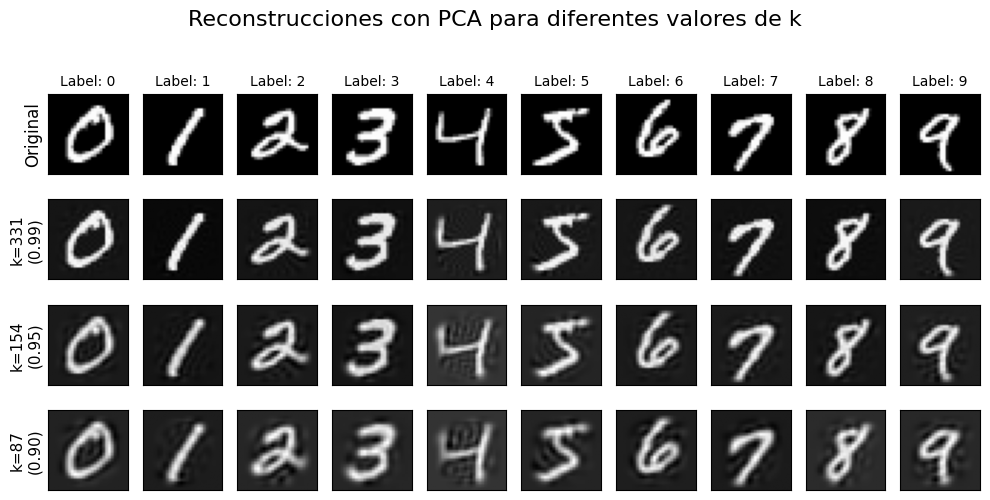
\includegraphics[width=0.9\textwidth]{figuras/pca_reconstructions.png}
    \caption{Reconstrucción de dígitos con PCA para distintos valores de $k$. Primera fila: imágenes originales. Filas siguientes: reconstrucciones con $k=54$, $k=87$, y $k=156$.}
    \label{fig:pca_reconstructions}
\end{figure}

También se realizó un análisis adicional aplicando K-means al espacio latente de PCA, utilizando las 87 componentes principales que explican el $90\%$ de la varianza. Se estableció K=10 (igual al número de clases) para evaluar si los clusters formados coincidían con los dígitos reales. Como se observa en la matriz de confusión (Figura~\ref{fig:pca_confusion}), aunque los clusters capturan cierta estructura de los datos, existe confusión significativa entre dígitos similares. Por ejemplo, los dígitos 4, 7 y 9 tienden a mezclarse en los mismos clusters debido a sus similitudes estructurales. De igual manera, hay confusión entre los dígitos 3, 5 y 8. Esto demuestra que, si bien la reducción de dimensionalidad preserva gran parte de la información visual, algunas distinciones sutiles entre ciertos dígitos requieren más componentes o técnicas más sofisticadas para ser capturadas correctamente.

\begin{figure}[H]
    \centering
    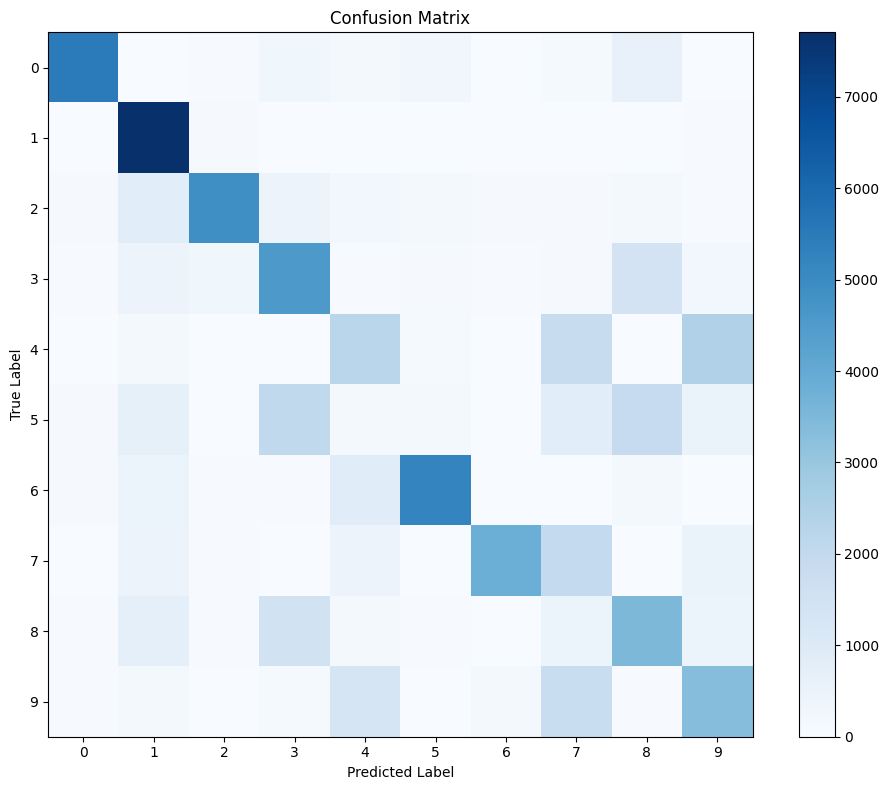
\includegraphics[width=0.7\textwidth]{figuras/matriz_de_cofuncion.png}
    \caption{Matriz de confusión resultante del análisis en el espacio latente de PCA.}
    \label{fig:pca_confusion}
\end{figure}

Por último, se proyectaron las imágenes al plano formado por las dos primeras componentes principales. En la Figura~\ref{fig:pca_2d} se observan los clusters formados por cada clase. Dos componentes no son suficientes para separar todos los numeros pero explican la estructura principal de cada numero. Podemos ver que se forman diferentes sub grupos de datos, los numero 4, 7 y 9 por ejemplo tienen una estructura similar y son proyectados al mismo espacio, mientras que los numeros 2, 3, 5, 6 y 8 forman otro grupo. Estos grupos coinciden con los nombrados antes en la matriz de confusión.

\begin{figure}[H]
    \centering
    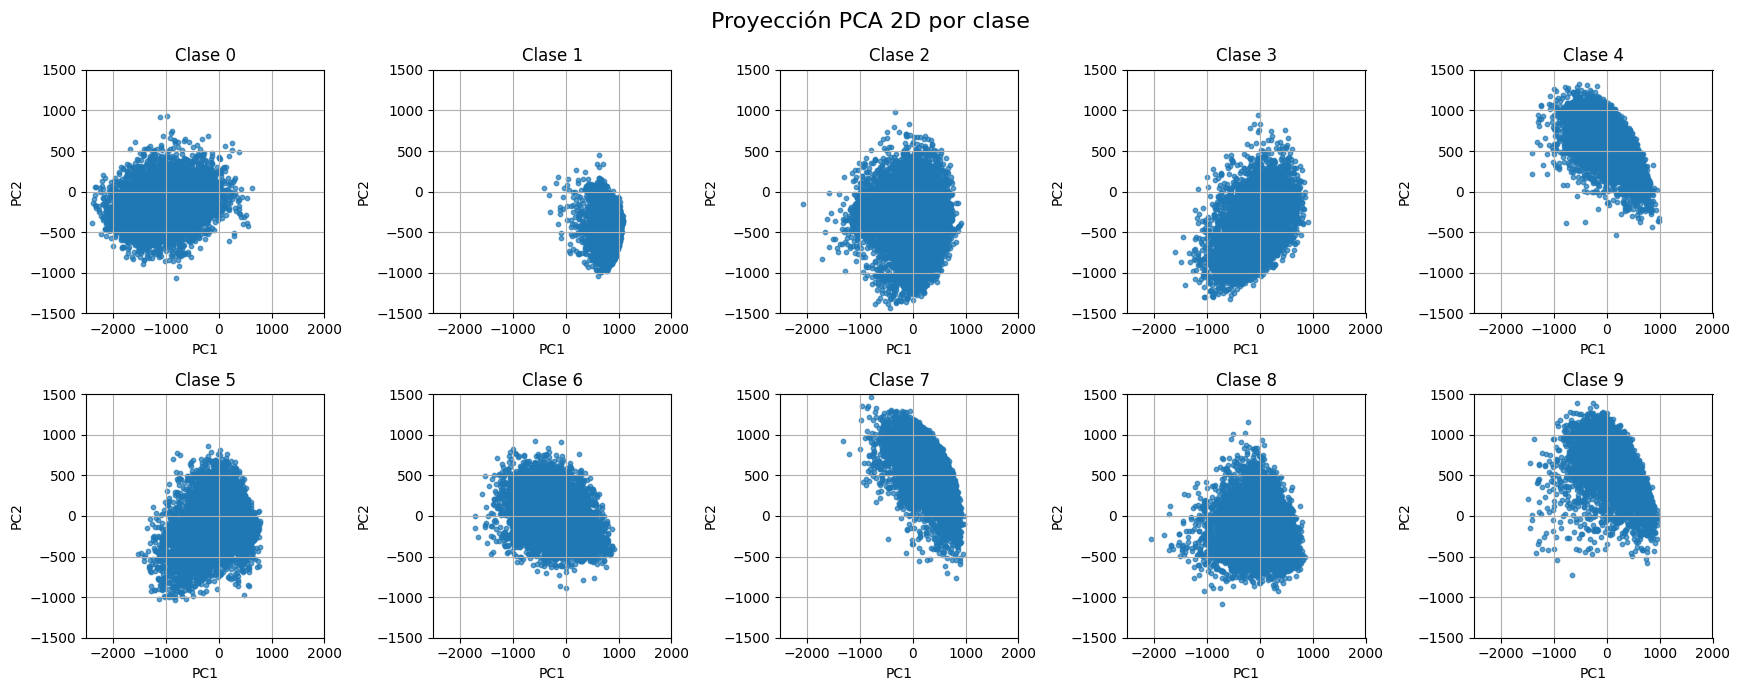
\includegraphics[width=\textwidth]{figuras/pca_2d.png}
    \caption{Visualización en 2D del dataset proyectado con las dos primeras componentes principales. Cada gráfico representa una clase de dígito.}
    \label{fig:pca_2d}
\end{figure}

Para analizar esta proyección, se calcularon las medias de cada clase en el espacio de las dos primeras componentes principales. Esto permite observar cómo se distribuyen los diferentes dígitos en este espacio reducido y facilita la identificación de patrones. Si reconstruimos las imagenes desde este espacio latente, de dos dimensiones, vamos a ver que el modelo se confunde mucho entre los numeros de su mismo sub grupo.

\begin{figure}[H]
    \centering
    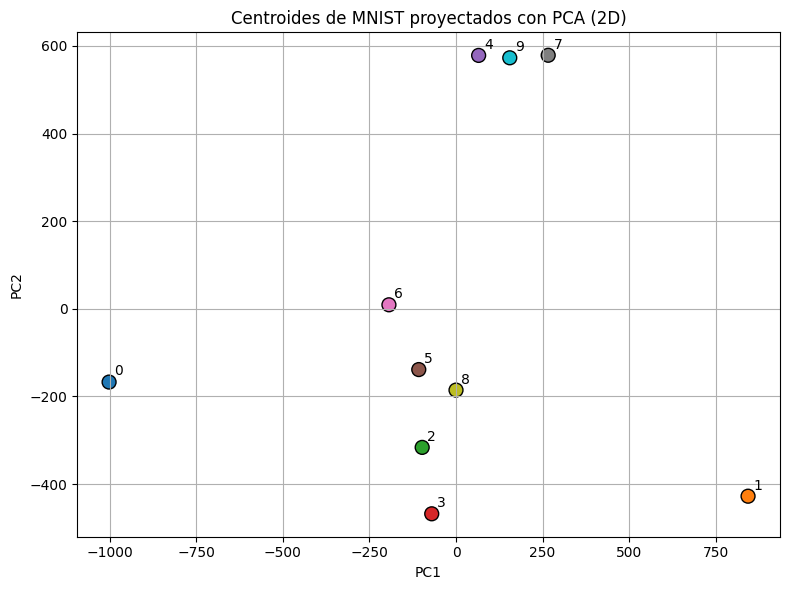
\includegraphics[width=0.7\textwidth]{figuras/pca_2d_medias.png}
    \caption{Análisis PCA: visualización en 2D de las medias de cada clase.}
    \label{fig:pca_medias}
\end{figure}

\section{Conclusiones}

En este trabajo se exploraron dos técnicas fundamentales del aprendizaje no supervisado: clustering y reducción de dimensionalidad. Ambas técnicas permiten extraer patrones y estructuras subyacentes en los datos sin necesidad de etiquetas previas.

En el análisis de clustering, se compararon tres algoritmos con características distintivas. K-means resultó efectivo para identificar agrupaciones esféricas, encontrando un punto óptimo en K=15 según el criterio del codo. GMM extendió este enfoque modelando distribuciones gaussianas, permitiendo mayor flexibilidad en la forma de los clusters. DBSCAN demostró ser particularmente útil para detectar agrupaciones de forma arbitraria y manejar ruido, aunque su desempeño depende crucialmente de la elección de parámetros $\varepsilon$ y $MinPts$.

En cuanto a la reducción de dimensionalidad mediante PCA aplicado al conjunto MNIST, se logró una compresión significativa de la información. Se determinó que con aproximadamente 87 componentes principales se puede explicar el 90\% de la varianza total, 154 componentes para el 95\%, y 331 para el 99\%. Esto representa una reducción sustancial frente a las 784 dimensiones originales, manteniendo la calidad visual de las imágenes reconstruidas.

La proyección de los dígitos en las dos primeras componentes principales reveló agrupaciones naturales, donde dígitos con estructuras similares (como 4, 7 y 9) tienden a proyectarse en regiones cercanas del espacio reducido. La matriz de confusión del clustering realizado en el espacio latente de 87 dimensiones (90\% de varianza explicada) confirmó estas similitudes estructurales, evidenciando que incluso con una representación que conserva la mayor parte de la información, persiste cierta confusión entre clases con características visuales similares.

Estos resultados subrayan la importancia de seleccionar el algoritmo y los parámetros adecuados según las características específicas de los datos y los objetivos del análisis. Las técnicas de aprendizaje no supervisado proporcionan herramientas valiosas para explorar y comprender la estructura intrínseca de los datos cuando no se dispone de etiquetas, facilitando posteriores tareas de análisis, clasificación o representación compacta de la información.

\end{document}




